\chapter{Avaliação de resultados}
\label{chap:eval}

A avaliação de algoritmos de classificação (e de aprendizagem de máquina em geral) é um tópico controverso, que é objeto de discussão de diversos trabalhos. Segundo um teorema da aprendizagem de máquina conhecido como "\emph{no free lunch}", algoritmos de aprendizagem têm performance igual quando comparados utilizando todos os possíveis conjuntos de dados. Ou seja, um algoritmo que é melhor aplicado a um domínio o faz somente abrindo mão de outros domínios.

Assim, a comparação simples desses algoritmos não tem valor prático. \citeauthor{Brownlee2007} nota que que muitos (ou a maioria) dos trabalhos foca apenas na qualidade da solução, que é apenas um aspecto da eficácia. Segundo \citeauthor{Barr1995}, existem diversos aspectos que devem ser considerados na avaliação de um método: eficiência, eficácia, robustez, complexidade, impacto, potencial para generalização e inovação \cite{Barr1995}. Em seu trabalho, os autores apresentam os passos básicos para a experimentação, conforme a listagem abaixo:

\begin{enumerate}[a)]
    \item Definir os objetivos do experimento
    \item Selecionar uma medida de performance e os fatores a serem explorados
    \item Planejar e executar o experimento
    \item Analisar os dados e tirar conclusões
    \item Divulgar os resultados do experimento
\end{enumerate}

Além disso, sugerem, no mesmo trabalho, diretrizes de alto-nível para o formato de divulgação dos resultados:

\begin{enumerate}[a)]
    \item O experimento deve ser facilmente reproduzido
    \item Todos os fatores que influenciam os resultados dever ser listados (código, ambiente de execução, etc)
    \item As medições devem ser precisas
    \item Os parâmetros devem ser especificados
    \item Comparações com outros métodos
    \item Reduzir a variabilidade dos resultados
    \item Garantir que os resultados são abrangentes
\end{enumerate}

Com isso em mente, é importante considerar as características únicas do domínio onde o método é aplicado. Os dados nos problemas de detecção de fraude apresentam desafios únicos que devem ser levados em consideração durante o desenvolvimento de um sistema de detecção, conforme apresentado na seção \ref{sec:fraud_data}.

\section{Detecção de fraude}
\label{sec:eval_fraud}

Phua e outros autores listam as diversas medidas de performance utilizadas em trabalhos recentes na área de detecção de fraude \cite{Phua2010}. Em relação à comparação da eficácia dos métodos, destacam-se os seguintes critérios:

\begin{enumerate}[a)]
    \item Similaridade de uma instância com os exemplos de fraude conhecidos divida pela dissimilaridade com exemplos legais.
    \item Análise da curva ROC (\emph{Receiver Operating Characteristic}, Característica de Operação do Receptor): a taxa de verdadeiros positivos para falsos positivos.
    \item Análise da área sob a curva ROC, que mede a probabilidade de uma instância positiva ser classificada como "mais positiva" do que uma instância negativa.
    \item Entropia cruzada: mede a diferença entre o valor atribuído na classificação de uma instância e o valor real atribuído àquela instância nos dados de teste.
    \item Escore Brier: o erro quadrático médio, ou seja, a média do somatório dos quadrados da diferença entre a classificação de uma instância e a classificação real.
    \item Alguns trabalhos adotam um critério peculiar: as instâncias são classificadas de acordo com o seu valor monetário. Esse valor pode ser tanto explícito quanto baseado em modelos financeiros.
\end{enumerate}

Em relação à eficiência dos métodos, destacam-se os seguintes critérios:

\begin{enumerate}[a)]
    \item Velocidade de detecção (tempo até o alarme).
    \item Número de tipos ou estilos de fraude detectados.
    \item Processo de de detecção em tempo real ou em lote.
\end{enumerate}

Os métodos tradicionais de medição, como a taxa de positivos (número de fraudes detectadas corretamente dividido pelo número de fraudes verdadeiras) e a precisão a um determinado limite (número de instâncias classificadas corretamente, dividido pelo número total de instâncias) foram abandonados pelos trabalhos recentes, devido à natureza peculiar da detecção de fraude.

A razão para isso é que o custo das classificações errôneas, no caso da detecção de fraude, são irregulares, incertos, variam de exemplo a exemplo e podem variar conforme o tempo. Falsos negativos são geralmente mais custosos do que falsos positivos. Um falso positivo geralmente leva apenas a uma verificação desnecessária por um especialista. Um falso negativo, no entanto, acarreta em uma fraude que não é detectada pelo sistema e não será reportada, deixando o fraudador impune. Mesmo assim, muitos dos sistemas de detecção comerciais, como a maioria dos departamentos governamentais que atuam na área de detecção de fraude, utilizam valores monetários como medida de avaliação \cite{Phua2010}.

\section{Avaliação dos modelos}

A primeira parte na avaliação de um algoritmo de classificação é a avaliação dos modelos criados por ele. Um modelo é a saída de um algoritmo de classificação ou a estrutura intermediária utilizada por ele, e define como as instâncias serão classificadas. O modelo é então aplicado a cada uma das instâncias da base de dados e gera uma classificação dessas instâncias.

Essa classificação pode ser comparada com as classificações verdadeiras das instâncias, gerando um total de instâncias classificadas corretamente. Esse valor é comumente representado como uma porcentagem, um valor entre 0 e 1, calculado como \emph{1 - taxaDeErros} e é chamado de \emph{precisão}.

\subsection{\emph{Holdout}}

Quando um modelo é criado à partir de um conjunto de dados e os testes são executados sobre esse mesmo conjunto, é muito provável que eles apresentem um bom resultado. No entanto, isso não garante que o modelo pode ser aplicado com a mesma eficácia sobre novos dados, o que geralmente é o objetivo dos sistemas de detecção. Para isso, o conjunto de dados é dividido em dados de treinamento e de testes.

O resultado dos testes pode ser altamente dependente dessa separação dos dados. Separar os dados de forma diferente geralmente altera o resultado dos testes. Para evitar essa dependência, foram criados métodos como \emph{holdout} e \emph{cross-validation}.

Para que seja possível avaliar se um modelo pode prever novos dados após o treinamento, a base de dados deve ser dividida em duas partes: um conjunto de treinamento e um conjunto de teste. O modelo é criado utilizando apenas os dados de treinamento e avaliado utilizando os dados de teste. Essa técnica é denominada \emph{holdout}, porque uma parte dos dados é retirada do processo de treinamento para que possa ser utilizada nos testes. Os resultados podem ser melhorados executando várias iterações de \emph{holdout}, dividindo um conjunto de dados aleatoriamente a cada vez e calculando a média e o desvio padrão da precisão.

Caso o resultado dos testes de um modelo quando aplicado aos mesmos dados utilizados no treinamento seja bom, mas o resultado quando aplicado aos dados de teste sejam ruins, diz-se que ocorre \emph{overfitting}: o modelo ajusta-se tanto aos dados de treinamento que não consegue criar regras genéricas o suficiente para identificar amostras semelhantes mas não exatamente iguais.

Há ainda a possibilidade do modelo não gerar um resultado bom nem mesmo para os dados de treinamento. Nesse caso, diz-se que ocorre \emph{underfitting}: o modelo não é capaz de criar regras que se ajustem aos dados de treinamento, ou seja, o modelo não é capaz de memorizar os dados de treinamento.

\subsection{\emph{Cross-validation}}
\label{sec:eval_cross_validation}

Uma alternativa mais sofisticada e eficiente do \emph{holdout} é denominada \emph{cross-validation}. Nela, os dados são divididos em \emph{n} partições, chamadas de \emph{folds}. A cada iteração, uma partição é utilizada dados de testes, enquanto as outras \emph{n - 1} são utilizadas como treinamento.

\begin{enumerate}[a)]
    \item Dividir aleatoriamente os dados em dois conjuntos, treinamento e testes.
    \item Criar o modelo com base no conjunto de dados de treinamento.
    \item Testar o modelo utilizando o conjunto de dados de testes.
    \item Repetir os passos a) a c).
    \item Calcular a média e o erro padrão da média dos resultados de cada iteração.
\end{enumerate}

Uma alternativa à divisão aleatória dos dados, chamada de \emph{cross-validation} estratificada, é a divisão onde a proporção das classes em cada partição é a mesma do conjunto total de dados. Isso aumenta ainda mais a fidelidade do treinamento e dos testes. Obviamente, esse método só pode ser utilizado em conjuntos de dados que contém um atributo de classe (ou seja, supervisionados).

Quando um conjunto de dados é pequeno, pode-se utilizar um tipo de \emph{cross-validation} chamado \emph{leave-one-out}, onde \emph{n}, o número de partições, é igual ao número de instâncias no conjunto de dados (ou seja, cada partição tem tamanho 1). Assim, a cada iteração, \emph{n - 1} instâncias são usadas no treinamento e o teste é feito sobre a instância restante.

\subsection{\emph{Grid search}}

O \emph{grid search} é outra técnica desenvolvido para diminuir o efeito de fatores não relacionados ao algoritmo na execução dos testes. Assim como o \emph{cross-validation} diminui o efeito da separação do conjunto de dados em dados de treinamento e de teste, o \emph{grid search} diminui o efeito da escolha dos parâmetros para o algoritmo. Esses parâmetros são valores numéricos ou condições que alteram o funcionamento da classificação das instâncias. Os algoritmos podem ter seu comportamento alterado através de parâmetros. Um exemplo disso é um classificador que aceita apenas valores maiores do que um determinado limiar. Diminuir ou aumentar esse limiar faz com que mais ou menos valores sejam aceitos.

Consequentemente, alterar o valor de um parâmetro afeta a precisão do classificador. Modelos mais complexos podem ter diversos parâmetros, e a relação entre estes pode também afetar a precisão. O treinamento é, então, dependente do valor dos parâmetros de um modelo. No entanto, esses parâmetros não são facilmente configuráveis, devido a dependências não-lineares que existem entre eles, que formam um sistema complexo. Os parâmetros podem também ser dependentes de contexto: parâmetros que geram um bom resultado para um determinado conjunto de dados podem não gerar um resultado tão bom para outro conjunto.

O \emph{grid search} consiste em executar e comparar a execução do algoritmo utilizando diversos valores para os parâmetros, para decidir qual é a melhor combinação para um conjunto de dados específico. \emph{Grid search} é um processo de diversas iterações de \emph{cross-validation} utilizando diferentes valores para os parâmetros de um modelo. No entanto, como os valores dos parâmetros podem ser dependentes entre si (e geralmente são), devem ser testadas todas as combinações de valores para cada e entre cada parâmetro. Esse é um processo computacionalmente custoso, já que o número de combinações é uma função exponencial do número de parâmetros e do número de valores distintos de cada parâmetro. Além disso, alguns parâmetros podem ter um número infinito de valores, como é o caso para parâmetros que são números reais.

Para resolver esse problema, no \emph{grid search} são utilizados um conjunto finito de valores para cada parâmetro. Esse conjunto é geralmente uma faixa de valores organizada em uma progressão aritmética, geométrica ou exponencial. Dessa forma é possível reduzir o conjunto (potencialmente infinito) de combinações possíveis para um tamanho razoável, através de um comprometimento no número de valores testados.

O resultado de um \emph{grid search} é a lista de resultados para a execução do algoritmo utilizando cada combinação de parâmetros e os resultados. Dessa forma, é possível utilizar a combinação de parâmetros que gera o melhor resultado.

É importante notar que o \emph{grid search} é um processo facilmente paralelizável. Considerando que um algoritmo aceite dois parâmetros, e cada um desses parâmetros tenha 3 valores possíveis, cada uma das 9 combinações possíveis é testada. Como cada teste é independente do outro, pode-se executar até 9 processos ao mesmo tempo. Caso a divisão aleatória dos dados nas iterações do \emph{cross-validation} seja calculada previamente, é possível que cada uma delas seja executada também em paralelo, aumentando ainda mais o número de processos simultâneos que podem ser executados.

\subsection{Dados baseados em tempo}

Uma característica importante de algumas áreas da detecção de fraude é que os dados são baseados em tempo, ou seja, o momento em que os dados de uma instância foram coletados é um atributo importante daquela instância. Para esse tipo de base de dados, é interessante que o treinamento seja feito utilizando dados mais antigos, e os testes utilizando dados recentes. Dessa maneira, é possível detectar se existe uma evolução nos dados conforme o tempo.

A razão para isso é que, caso os dados sejam misturados aleatoriamente, a informação da evolução dos padrões é perdida durante o treinamento. Caso sejam utilizados dados recentes para os testes, essas alterações podem ser detectadas caso haja uma variação entre os resultados dos testes nos dados de treinamento (antigos) e de testes (recentes).

Caso essa diferença seja detectada, uma solução para adicionar essa informação ao modelo é aplicar um peso sobre as instâncias de acordo com o tempo. Assim, instâncias mais recentes teriam mais importância para o treinamento do que instâncias mais antigas. Deve ser utilizado um balanceamento para essa solução, já que utilizar todos os dados disponíveis (incluindo os dados recentes) torna o modelo mais completo, mas torna impossível avaliar com segurança a eficácia desse modelo.

\section{Avaliação de classificadores}

Na área de detecção de fraude, geralmente se lida com classificadores binários. Classificadores binários são aqueles que, para um dado conjunto de valores de entrada, geram como valor de saída um valor Booleano: verdadeiro ou falso, positivo ou negativo. Os sistemas de detecção de fraude se situam, na maioria dos casos, nessa categoria: os dados referentes a uma instância passam pelo sistema de detecção e são classificados como legítimos ou fraudulentos \cite{Bewick2004}. Sistemas mais complexos podem gerar saídas com mais informações sobre a instância, como o grau de certeza da previsão ou o grau de semelhança entre a instância e os dados da base.

Como exemplo, inspirado em \citet{Bewick2004}, é apresentado nessa seção um sistema de detecção de fraude, que considera como único atributo das instâncias o número de ocorrências de um determinado valor. Nesse ambiente simplificado, a instância é considerada fraudulenta caso um limiar de ocorrências seja ultrapassado.

Esse sistema de testes utiliza como único critério de avaliação o número de ocorrências. Um \emph{limiar de classificação} é definido: um parâmetro que o sistema de detecção utilizará para guiar a previsão da detecção. Se o limiar de classificação fosse 1, todas as instâncias que tivessem mais de uma ocorrência (nos valores de exemplo, as instâncias 0 e 2) seriam consideradas fraudulentas.

\renewcommand{\arraystretch}{1.5}
\begin{table}[h]
    \vspace{0.5cm}
    \centering
    \caption{Exemplo de resultado}
    \label{fraud:ex}
    \vspace{0.5cm}
    \begin{tabular}{c l c c c}
        & & \multicolumn{2}{c}{\textbf{Dados reais}} \\
        \multirow{3}{5mm}{\begin{sideways}\parbox{20mm}{\textbf{Saída}}\end{sideways}} & \multicolumn{1}{c|}{} & Fraude & Legítimo & \multicolumn{1}{|c}{Total} \\
        \cline{2-5}
        & \multicolumn{1}{c|}{Fraude}   & 300 & 200   & \multicolumn{1}{|c}{500}  \\
        & \multicolumn{1}{c|}{Legítimo} & 100 & 1000  & \multicolumn{1}{|c}{1100} \\
        \cline{2-5}
        & \multicolumn{1}{c|}{Total}    & 400 & 1200  & \multicolumn{1}{|c}{1600} \\
    \end{tabular}
    \vspace{0.5cm}
\end{table}

Um exemplo do resultado de um teste nesse sistema é mostrado na tabela \ref{fraud:ex}. As colunas sob ``Dados reais'' mostram o número de instâncias fraudulentas e legítimas; as linhas sob ``Saída'' mostram a classificação gerada pelo sistema. A partir desses dados, a avaliação dos resultados é feita usando dois conceitos: sensibilidade e especificidade.

\subsection{Matriz de confusão}

A avaliação dos classificadores binários é feita com base em uma \emph{matriz de confusão}, conforme mostrado na tabela \ref{fraud:confusion}. Nessa tabela são listados o número de valores (ou porcentagem) para cada combinação de saída do sistema e a classificação real. Instâncias corretamente classificadas ocupam as colunas Positivo e Negativo, enquanto instâncias cujo classificação difere da realidade ocupam as colunas ``Falsos positivos'' e ``Falsos negativos''.

\renewcommand{\arraystretch}{1.5}
\begin{table}[h]
    \vspace{0.5cm}
    \centering
    \caption{Matriz de confusão}
    \label{fraud:confusion}
    \vspace{0.5cm}
    \begin{tabular}{c l c c}
        & & \multicolumn{2}{c}{\textbf{Dados reais}} \\
        \multirow{3}{5mm}{\begin{sideways}\parbox{20mm}{\textbf{Saída}}\end{sideways}} & \multicolumn{1}{c|}{} & Positivo & Negativo \\
        \cline{2-4}
        & \multicolumn{1}{c|}{Positivo} & Positivo & Falso positivo\\
        & \multicolumn{1}{c|}{Negativo} & Falso negativo & Negativo\\
    \end{tabular}
    \vspace{0.5cm}
\end{table}

Como o conjunto de dados possui apenas duas classes, a matriz de confusão é $2 x 2$, mas o número de linhas e colunas pode ser maior, sendo igual ao número de classes. Todos os principais indicadores podem ser extraídos através da matriz de confusão, fazendo dela uma forma sucinta de apresentação dos resultados.

A diagonal principal representa as instâncias corretamente classificadas (\emph{i.e.} instâncias positivas classificadas como positivas, negativas classificadas como negativas). Todas as outras células da matriz são instâncias incorretamente classificadas, onde o cruzamento do nome da coluna e da linha mostra a classificação gerada pela algoritmo e a classificação real. Através dos elementos da diagonal principal, é possível calcular:

\begin{enumerate}[a)]
    \item \emph{Taxa de positivos verdadeiros (TP)\nomenclature{TP}{Taxa de positivos verdadeiros}}: a proporção das instâncias classificadas como \emph{x} entre todas as que realmente fazem parte da classe \emph{x}, calculada dividindo o elemento da classe na diagonal principal pela soma dos elementos na mesma linha. Também é conhecida como \emph{recall}.
    \item \emph{Taxa de falsos positivos (FP)\nomenclature{FP}{Taxa de falsos positivos}}: a proporção das instâncias classificadas como \emph{x} que na verdade pertencem a outra classe entre todas as que não fazem parte da classe {x}, calculada subtraindo o elemento da classe na diagonal principal da soma dos elementos na mesma coluna e dividindo o valor resultante pela soma dos elementos nas linhas de todas as outras classes.
    \item \emph{Precisão}: a proporção de instâncias que fazem parte da classe \emph{x} entre todas as que foram classificadas como \emph{x}, calculada dividindo o elemento da classe na diagonal principal pela soma dos elementos na mesma coluna.
    \item \emph{\emph{F-measure}}: uma combinação da precisão e taxa de positivos verdadeiros, calculada através da média harmônica da precisão e \emph{recall}, 2 * (precisão * \emph{recall}) / (precisão + \emph{recall}).
\end{enumerate}

\subsection{Sensibilidade e especificidade}

\emph{Sensibilidade} refere-se à proporção de instâncias corretamente classificadas como positivas. \emph{Especificidade} refere-se à proporção de instâncias corretamente classificadas como negativas. Tomando como exemplo os dados da tabela \ref{fraud:ex}, a sensibilidade é igual a 300 / 400 = 0.75; e a especificidade é igual a 1000 / 1200 = 0.8333. Ou, visto de outra maneira, 75\% das fraudes foram realmente classificadas como fraudes; e 83.33\% das instâncias legítimas foram classificadas como legítimas.

Apenas a consideração desses dois valores pode levar a uma correta avaliação dos resultados do teste, principalmente nos domínios da detecção de fraude. Uma alta sensibilidade não necessariamente implica em uma alta especificidade, e vice versa. Dessas duas informações são derivados os \emph{valores preditivos positivos e negativos}.

\subsection{Valores preditivos}

O \emph{valor preditivo positivo} é a chance de uma instância ser realmente uma fraude caso seja classificada como tal pelo sistema. O \emph{valor preditivo negativo} é a chance de uma instância ser realmente legítima caso seja classificada como tal pelo sistema. Para os dados de exemplo, o valor preditivo positivo é 300 / 500 = 0.6; e o valor preditivo negativo é 1000 / 1100 = 0.9091. Ou, visto de outra maneira, 60\% das instâncias que foram classificadas como fraude eram realmente fraudes, e 90.91\% das instâncias classificadas como legítimas eram realmente legítimas.

Esses dois valores são o oposto da sensibilidade e especificidade, respectivamente. Enquanto os valores preditivos dão uma avaliação direta sobre os resultados dos testes, a sensibilidade e especificidade não são afetadas pela proporção dos valores nas instâncias, ou seja, não são alteradas quando há uma alteração na proporção de fraudes.

\subsection{Taxas de verossimilhança}

A sensibilidade e especificidade tornam-se ainda mais úteis quando combinadas, gerando as taxas de verossimilhança. A taxa de verossimilhança de um resultado positivo (LR\textsuperscript{+}) é a razão entre a probabilidade de um resultado positivo no teste caso a instância seja realmente positiva (coluna "positivo" da matriz de confusão) e a probabilidade de um resultado positivo no teste caso a instância seja na verdade negativa:

\begin{equation}
    \vspace{2mm}
    LR^{+}=\frac{sensibilidade}{1 - especificidade}
    \vspace{2mm}
\end{equation}

No exemplo, LR\textsuperscript{+} = 0.75 / (1 - 0.8333) = 4.4991. Isso significa que um resultado positivo nos testes é 4.4991 vezes mais provável para instâncias que são realmente positivas do que para aquelas que não são.

De maneira, similar, a taxa de verossimilhança negativa (LR\textsuperscript{-}) é a razão entre a probabilidade de um resultado negativo no teste caso a instância seja realmente negativa (coluna "negativo" da matriz de confusão) e a probabilidade de um resultado negativo no teste caso a instância seja na verdade positiva:

\begin{equation}
    \vspace{2mm}
    LR^{-}=\frac{1 - sensibilidade}{especificidade}
    \vspace{2mm}
\end{equation}

No exemplo, LR\textsuperscript{-} = (1 - 0.75) / 0.8333 = 0.3, o que significa que um resultado negativo no teste é 0.3 vezes mais provável para instâncias que são realmente negativas do que para aquelas que não são.

Desses valores, pode-se atestar a utilidade do método para classificação. Uma alta taxa de verossimilhança positiva indica que o teste é útil para verificar se uma instância é positiva, enquanto uma alta taxa de verossimilhança negativa é útil para verificar se uma instância é negativa. Assim como os valores preditivos, essas taxas são sensíveis à predisposição dos dados na base de dados.

\subsection{Índice de Youden e ROC}

Os dados de teste do exemplo mostrados nas tabelas até agora consideraram apenas um valor como limiar de classificação. Mudanças nesse limiar afetam a precisão dos testes: caso o limiar seja seja igual a -1, todas as instâncias são classificadas como fraudulentas, já que todas possuem como número de ocorrências um número maior ou igual a zero. Por outro lado, caso o limiar seja um número maior do que qualquer uma das instâncias, todas serão classificadas como legítimas. Em sistemas reais, é comum que sejam testados diversos valores para esse limiar sobre uma mesma base de dados, para que o melhor seja identificado e usado no sistema final. A tabela \ref{fraud:youden} é um exemplo de resultados para esse tipo de teste.

\begin{table}[h!]
    \vspace{0.5cm}
    \centering
    \caption{Exemplo de resultados para testes comparativos de limiares}
    \label{fraud:youden}
    \vspace{0.5cm}
    \begin{tabular}{l c c c c c}
        \hline
        Limiar & Fraudes & Legítimos & Sensibilidade & Especificidade & Índice de Youden \\
        \hline
        0     & 400 &    0 & 1      & 0      & 0      \\
        1     & 395 &  400 & 0.9875 & 0.3333 & 0.3208  \\
        2     & 380 &  600 & 0.95   & 0.5    & 0.45   \\
        3     & 375 &  900 & 0.9375 & 0.75   & 0.6875 \\
        4     & 200 & 1000 & 0.5    & 0.8333 & 0.3333 \\
        99    &   0 & 1200 & 0      & 1      & 0      \\
        \hline
        Total & 400 & 1200 &    -   &    -   &    -   \\
        \hline
    \end{tabular}
    \vspace{0.5cm}
    \\ Fonte: inspirado em \citet{Bewick2004}.
    \vspace{0.5cm}
\end{table}

Uma medida para a avaliação dos diferentes limiares pode ser a sensibilidade e especificidade. O índice de Youden (J), que é uma derivação desses valores, é uma medida apropriada nesses casos (eq. \ref{fraud:yindex}). Esse índice é um valor normalizado na faixa [0, 1], onde 1 significa um teste perfeito, classificando todas as instâncias corretamente; e 0 significa um teste sem valor nenhum. A tabela \ref{fraud:yindex} mostra os valores para os resultados com diversos limiares. É importante notar como valores extremos maximizam a sensibilidade e a especificidade, mas apenas aqueles limiares que maximizam os dois valores recebem índices significativos.

\begin{equation}
    \vspace{2mm}
    J = sensibilidade + especificidade - 1
    \label{fraud:yindex}
    \vspace{2mm}
\end{equation}

Uma característica importante do índice de Youden é que ele estabelece uma equivalência na relevância dos falsos positivos e negativos. Quando um é mais relevante que o outro, devido à peculiaridades nos dados ou no domínio do problema, ele não é apropriado. Nesses casos, pode-se atribuir pesos diferentes a ambos os valores. Um exemplo de adaptação do cálculo do índice de Youden é mostrado abaixo. Nessa fórmula, os valores ainda são mantidos na mesma faixa, mas falsos positivos recebem o dobro da significância.

\begin{equation}
    \vspace{2mm}
    J = 0.75 * sensibilidade + 0.25 * especificidade
    \vspace{2mm}
\end{equation}

Como pode-se observar na tabela \ref{fraud:yindex}, alterações no valor usado na classificação alteram o número de instâncias classificadas como positivas e negativas. Geralmente os resultados são distribuídos começando com um grande valor de sensibilidade e um valor baixo de especificidade; esses valores convergem até um máximo global; e então terminam em com um valor baixo de sensibilidade e um grande valor de especificidade. A variação desses três valores, e a interação entre eles, é mostrada no gráfico da figura \ref{fraud:threshold}.

\begin{figure}[h!]
    \vspace{0.5cm}
    \centering
    \caption{Variação dos valores de avaliação conforme o limiar de detecção}
    \label{fraud:threshold}
    \vspace{0.5cm}
    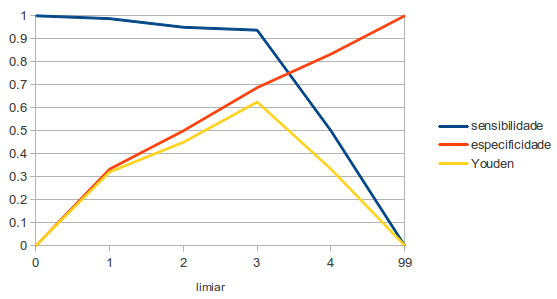
\includegraphics[scale=0.5]{img/threshold.png}
    \vspace{0.5cm}
\end{figure}

No lado esquerdo, onde o limiar é muito baixo, a sensibilidade é 1 e a especificidade, zero; enquanto no lado direito, onde o limiar é muito alto, ocorre o oposto: a sensibilidade é zero e a sensibilidade, 1. Conforme o limiar aumenta (começando do lado esquerdo e caminhando para a direita), ocorreu uma diminuição na especificidade (algumas instâncias fraudulentas começam a ser classificadas como legítimas). No entanto, há um aumento muito maior na especificidade (instâncias legítimas começam a ser classificadas corretamente). É possível ver como o índice de Youden mostra a real proporção entre esses dois valores. Uma forma mais sucinta para apresentar esse tipo de informação é através de um gráfico dos valores de sensibilidade e 1 - especificidade, que é denominado ROC (característica operativa do receptor, \emph{receiver operating characteristic}), conforme mostrado na figura \ref{fraud:roc}.

\begin{figure}[h!]
    \vspace{0.5cm}
    \centering
    \caption{Gráfico da curva ROC dos valores de exemplo}
    \label{fraud:roc}
    \vspace{0.5cm}
    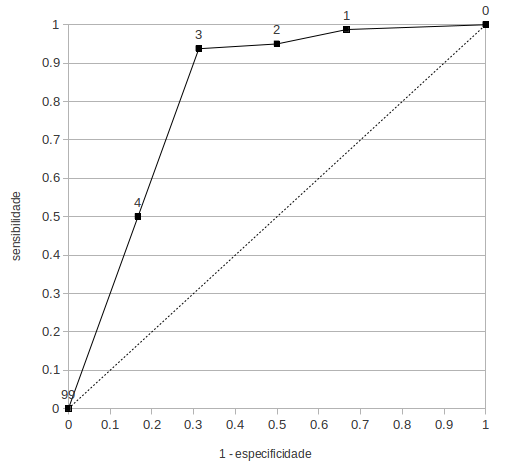
\includegraphics[scale=0.5]{img/roc.png}
    \vspace{0.5cm}
\end{figure}

No gráfico é visualmente aparente que o valor 3 como limiar de classificação oferece o melhor balanceamento entre sensibilidade e especificidade. Também é possível perceber como as alterações no limiar influenciam a distribuição desses dois valores. Um teste perfeito, que classificasse todas as instâncias corretamente, teria ambos os valores iguais a 1, tendo portanto um ponto no canto superior esquerdo do gráfico. Os pontos mais próximos dessa localização são aqueles que melhor classificam as instâncias.

Caso as instâncias fossem classificadas aleatoriamente, tendo chances iguais de serem classificadas tanto positivas quanto negativas, a sensibilidade e a especificidade seria ambas 0.5, e o teste não teria qualquer valor. Essa situação é representada pela linha diagonal entre os pontos (0, 1) e (1, 0). Essa linha é outro indicador visual útil: testes abaixo dela (na direção do canto inferior direito) têm muito pouco valor; testes próximos dela têm valor mediano; e testes acima (na direção do canto superior esquerdo) têm grande valor.

Uma das maneiras de quantificar a (dar um valor à) validade de um atributo como variável de diagnóstico é através do cálculo dá área sob a curva ROC (denominada AUROC, \emph{area under the ROC curve}). O teste ideal citado acima teria área igual a 1, enquanto testes completamente aleatórios teriam área 0.5. Testes reais normalmente situam-se entre esses dois valores, com valores mais próximos de 1 representando testes mais precisos.

O cálculo da área pode ser feito somando-se a área dos trapézios formados pela curva. Tomando dois pontos da curva, (0.1667, 0.5) e (0.3125, 0.9375), o trapézio formado por esses pontos e os pontos (0.1667, 0.0) e (0.3125, 0.0) é igual a (0.9375 - 0.5) x (0.3125 + 0.1667)/2 = 0.1048. Aplicando essa regra aos outros pontos da curva, obtêm-se uma área total de 0.8161, ou seja, uma instância fraudulenta tem 81.61\% de ter um número de ocorrências de inadimplência maior do que uma instância legítima.

\subsection{Comparação}

Uma vez que possa ser quantificada, a capacidade de diagnóstico de uma variável pode ser comparada com outras, simplesmente comparando-se as suas curvas ROC e as áreas sob essas curvas. Variáveis com uma maior área sob a curva geram diagnósticos mais confiáveis. O formato da curva também pode servir como instrumento de análise: uma variável pode ter comportamentos preferíveis caso as condições de teste sejam diferenciadas, ou para filtrar casos específicos. Por exemplo, uma variável que, para valores muito baixos de sensibilidade, apresenta uma alta taxa de especificidade pode ser usada quando quer-se favorecer a especificidade.

A área sob a curva ROC é um método útil para a medição da precisão de diagnósticos, além da comparação entre diferentes testes. No entanto, ela não deve ser tomada como verdade absoluta. A sensibilidade e a especificidade podem manter-se fixas em um ambiente de testes, mas podem variar conforme as características da população analisada.

Uma consideração importante quando analisa-se o desempenho de dois ou mais sistemas é que muito difícil (ou até mesmo impossível) excluir-se todos os fatores externos, resultando em uma análise completamente imparcial. Nesse caso específico, o resultado dos testes em cada algoritmo é fortemente influenciado pelas características dos dados na base de dados, embora os métodos de análise dos resultados procuram minimizar essa influência.

\subsection{Sistemas imunológicos artificiais}

Uma característica dos algoritmos inspirados na biologia é que eles tem um elemento estocástico, ou seja, em qualquer momento da sua execução, seu estado tem um elemento não-determinístico. Por isso, ao contrário dos métodos tradicionais, diversas execuções do treinamento podem apresentar resultados diferentes, mesmo quando os mesmos valores são usados para os parâmetros.

\section{Considerações finais}

A aplicação de critérios é vital para que um experimento possa ser analisado corretamente. Critérios não apropriados podem levar a informações erradas e conclusões que não seguem a realidade. Um exemplo clássico disso é um modelo que apresenta \emph{overfitting} (seção \ref{sec:eval_cross_validation}). Caso o modelo fosse testado apenas nos dados de treinamento, o resultado pareceria extremamente satisfatório. No entanto, o modelo apresentaria um desempenho péssimo em outros conjuntos de dados, o que tornaria-o inútil para qualquer aplicação.

Nos testes, a execução de cada algoritmos é feita utilizando \emph{grid search} e \emph{cross-validation}. Utilizar \emph{cross-validation} diminui a influência do conjunto de dados no resultado dos testes. Como o algoritmo é treinado e testado várias vezes, cada vez com uma divisão diferente do conjunto de dados para treinamento e testes, quaisquer tendências nos dados são eliminadas, e o resultado se torna mais confiável.

Geralmente, o \emph{grid search} é utilizado para selecionar os melhores parâmetros para um modelo, para que esses parâmetros sejam incorporados no sistema final, obtendo a melhor performance possível. Nesse trabalho, ele é utilizado para que o modelo utilizado nos testes seja o melhor possível para os conjuntos de dados dos testes.

Para a avaliação dos resultados, para cada algoritmo, são utilizados como critérios o erro médio relativo e o índice de Youden. O erro médio relativo é uma medida padrão simples, que mostra o quanto o resultado de um teste difere dos valores corretos. Ele é utilizado como uma métrica simples para o desempenho de um algoritmo, e pode ser utilizado como análise superficial na comparação de algoritmos. No entanto, o erro médio relativo não pode ser utilizado como métrica única: devido a simplicidade do seu cálculo, não é suficiente para a análise de áreas mais complexas como a detecção de fraude.

O índice de Youden é uma medida de performance que leva em consideração não só o número de instâncias classificadas corretamente. Para que o índice de Youden seja alto, tanto a taxa de falsos positivos quanto a de falsos negativos deve ser baixa. Conforme apresentado na seção \ref{sec:eval_fraud}, na detecção de fraude os falsos negativos são muito mais críticos do que os falsos positivos. Assim, serão calculados dois índices: o índice de Youden padrão e o índice de Youden com maior significância para os falsos negativos. Esse é calculado através da fórmula:

\begin{equation}
    \vspace{2mm}
    J = 0.25 * sensibilidade + 0.75 * especificidade
    \vspace{2mm}
\end{equation}

A partir do próximo capítulo é apresentado o desenvolvimento dos experimentos, tendo como base os conceitos apresentados nesse e nos capítulos anteriores.
